% \begin{algorithm}
%     \caption{Kernel PCA}
%     \label{alg:kernel-pca}
%     \KwIn{Data matrix \(A \in \RR^{n \times d}\), kernel function \(k\), number of components \(p \leq n\)}
%     \KwOut{Transformed data \(\tilde{A} \in \RR^{n \times p}\)}
% \end{algorithm}

Let \(x_1, x_2, \dots, x_n \in \RR^d\) be input vectors and \(k : \RR^d \times \RR^d \to \RR\) be a kernel.
The kernel PCA algorithm outputs the transformed input vectors \(\tilde{x}_1, \tilde{x}_2, \dots, \tilde{x}_n \in \RR^n\).
\begin{enumerate}
    \item Compute the kernel matrix \(K = [k(x_i, x_j)]_{ij}^{n \times n}\).
    \item Center kernel matrix \(K_0 = K - \colmean(K) - \rowmean(K) + \mean(K)\).
    \item Compute eigenvalues \((\lambda_j)_{j=1}^n\) and eigenvectors \((u_j)_{j=1}^n\) of \(K_0\) so that \(\lambda_1 \geq \lambda_2 \geq \cdots \geq \lambda_n\).
    \item Scale the eigenvectors to obtain the principal components in the RKHS: \(v_j = u_j / \sqrt{\lambda_j}\) for all \(j = 1,2,\dots,n\).
    \item Transformed points can be computed using
    \(y = \left[\vphantom{\Big|}\ipt{\vphantom{\big|}v_j, [k(x_i,x)]_{i=1}^n}\right]_{j=1}^n\).
\end{enumerate}

\begin{example}
    \label{eg:gaussian-kpca}
    Consider the problem of classifying points based on their radii.
    These points cannot be separated using a linear classifier in the two dimensions.
    However, by mapping them to a three-dimensional space, they can be separated by planes.
    Applying kernel PCA, these points can be sent to the RKHS associated with a Gaussian kernel without using an explicit feature map.
    The points in this high-dimensional feature space can then be projected onto the first three principal components to find separation boundaries.
    See \Cref{fig:gaussian-kpca-example}.
    \begin{figure}
        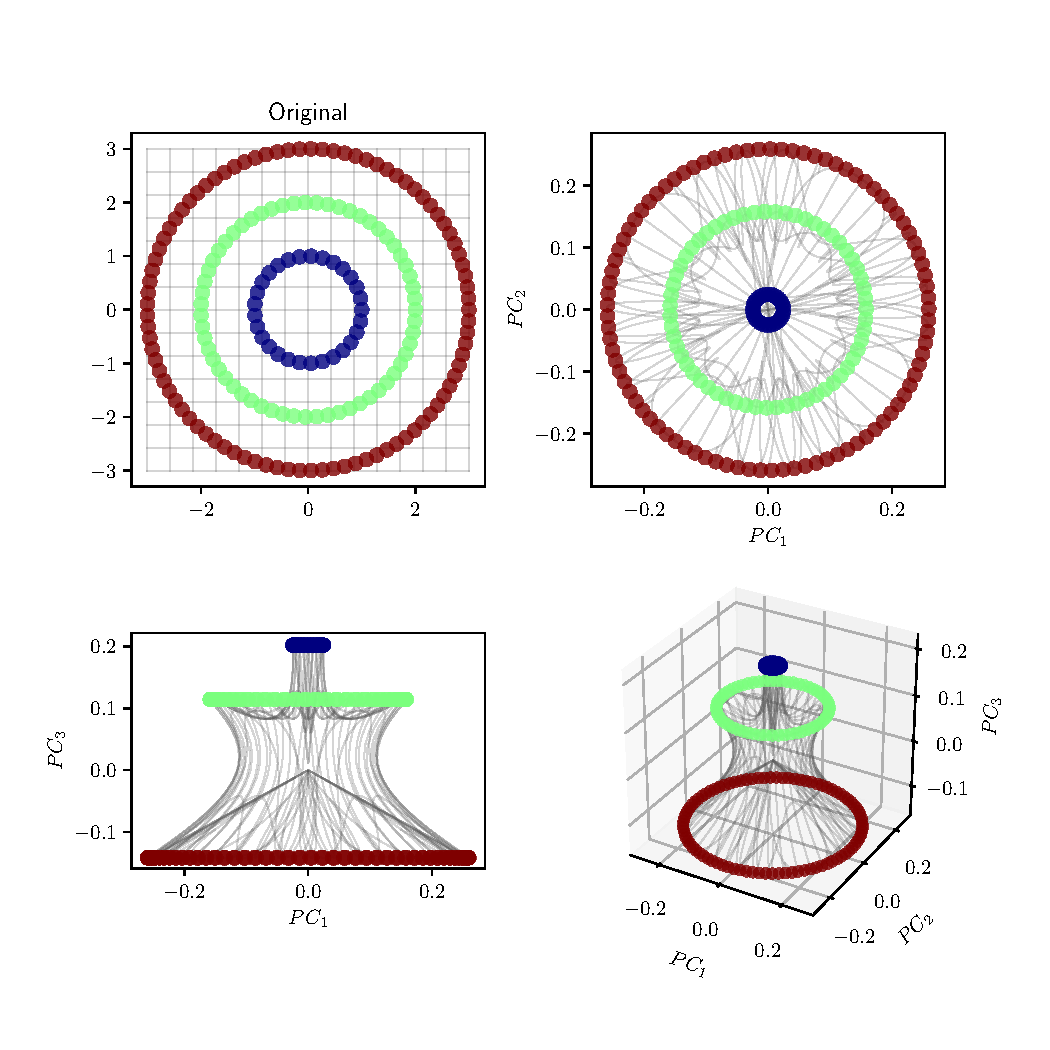
\includegraphics[width=\textwidth]{figs/fig_kpca_example.pdf}
        \caption{An idealized set of points in the plane are classified based on their radius. Kernel PCA with the Gaussian kernel is applied to find separation boundaries using the first three principal components.}
        \label{fig:gaussian-kpca-example}
    \end{figure}
\end{example}